\documentclass[a4paper, 11pt]{report}

\usepackage[latin1]{inputenc}
\usepackage[italian]{babel}
\usepackage{makeidx}
\usepackage{graphicx}

\title{\Huge\textbf{Elaborato\\di\\Programmazione Web}\\ \vspace{1cm} \huge Sito Web del Gruppo di Basi di Dati e Sistemi Informativi: Pubblicazioni e Corsi}
\author{\textit{Lorenzi Roberta} Matricola: 72361\and \textit{Piccinelli Andrea} Matricola: 83392}
\date{A.A. 2010--2011}

\begin{document}
\begin{figure}[t]
	\centering
	
\includegraphics[height=6cm, width=6cm]{logoUnibs.jpg}\\
	Universit� degli Studi di Brescia\\Facolt� di Ingegneria\\Corso di Laurea Magistrale in Ingegneria Informatica
\end{figure}
\maketitle

\tableofcontents

\chapter{Metodologia}
\newpage

\section{Analisi dei Requisiti}

\subsection{Descrizione problema, contesto dell'elaborato e requisiti richiesti}
L'elaborato tratta la ristrutturazione di due sezioni del sito web del Gruppo di Basi di Dati e Sistemi
Informativi, in particolare la sezione delle pubblicazioni e quella dei corsi.\\
\\
\textit{Descrizione Problema}: La gestione delle pubblicazioni e dei corsi, nel portale preesistente, 
� non strutturata ed � anzi basata su un sistema di archiviazione su file di testo. Inoltre non esiste
un'interfaccia di back-office che permetta l'immissione e la modifica di questi dati.\\
Questa struttura comporta un notevole lavoro per la modifica di corsi gi� esistenti o la creazioni di 
nuovi, cos� come per l'immissione di nuove pubblicazioni o la loro modifica.\\
\\
\textit{Contesto}: Attualmente la sezione del portale relativa a pubblicazioni � divisa fra le seguenti
tipologie:
\begin{itemize}
\item Pubblicazioni su riviste internazionali
\item Capitoli in libro
\item Pubblicazioni in atti di congressi (divise ulteriormente per anno)
\end{itemize}
I corsi sono invece divisi per facolt� in cui vengono svolti e hanno la seguente struttura generale:
\begin{itemize}
\item Titolo del corso e anno accademico
\item Docenti che tengono il corso
\item Corso/i di studio a cui si rivolge il corso
\item News
\item Orario delle lezioni e di ricevimento
\item Obiettivi del corso
\item Programma d'esame
\item Materiale di riferimento
\item Materiale didattico diviso in diverse sezioni (Lucidi lezioni, Lucidi esercitazioni, ...)
\end{itemize}
Il problema � nato quindi dall'esigenza di avere la comodit� di un'interfaccia web chiara, semplice 
e veloce per la gestione degli inserimenti e della modifica di pubblicazioni e di corsi.\\
\\
\textit{Requisiti richiesti}: Viene richiesta la realizzazione di un database per l'archiviazione dei 
dati che verranno inseriti. Inoltre deve essere realizzata un'interfaccia web per l'inserimento di 
pubblicazioni e corsi in modo semplice e strutturato.\\
Per quanto guarda le pubblicazioni le tipologie da considerare sono le seguenti:
\begin{itemize}
\item Pubblicazioni su riviste internazionali
\item Capitoli in libro
\item Pubblicazioni in atti di conferenza
\item Monografie
\item Curatele
\end{itemize}
Per i corsi di studio la struttura generale resta quella attuale.\\
\\
Sono stati realizzati dei mockup della struttura delle pagine da realizzare, sia per le pubblicazioni
che per i corsi.\\

\newpage
\subsubsection{Mockup Pubblicazioni}
\textbf{1 - Pubblicazioni su Riviste}
\begin{figure}[ht]
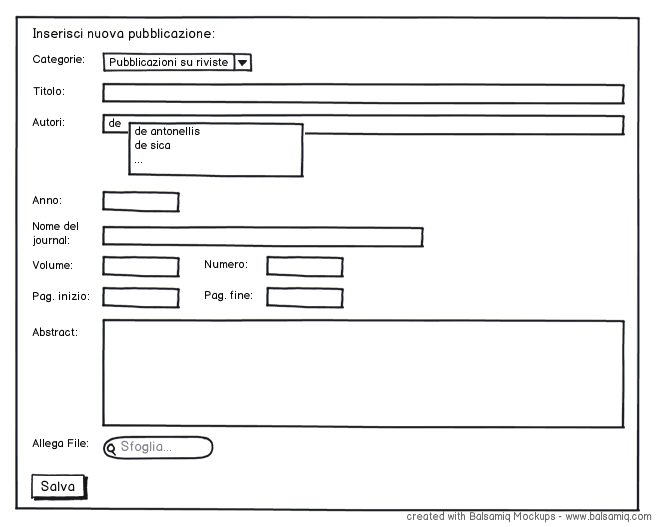
\includegraphics[height=10cm]{Mockup/Pubblicazioni/Image/PubblicazioniRiviste.png}
\caption{Pubblicazioni su Riviste \label{nome}}
\end{figure}
\\
\textit{Caratteristiche:}
\begin{itemize}
\item Autori: sono da scegliere da una lista che si genera con nuovi inserimenti
\item Nome del journal: da scegliere da una lista che si genera con nuovi inserimenti
\item Volume e numero sono numerici e devono essere visualizzati nella forma Volume(numero): esempio
43(8) volume = 43 numero = 8. Se il numero non � presente va visualizzato solo il Volume
\end{itemize}
I campi sono tutti obbligatori tranne 'Abstract', 'Numero' e l'allegare un file.
\clearpage

\textbf{2 - Capitoli in libro}
\begin{figure}[ht]
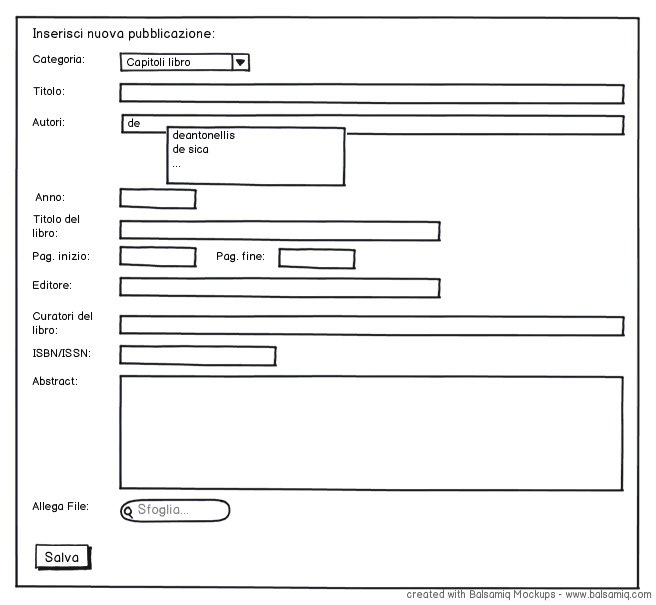
\includegraphics[height=11cm]{Mockup/Pubblicazioni/Image/CapitoliLibro.png}
\caption{Capitoli in libro \label{nome}}
\end{figure}
\\
\textit{Caratteristiche:}
\begin{itemize}
\item Autori: sono da scegliere da una lista che si genera con nuovi inserimenti
\item Curatore del libro: quando viene visualizzata deve essere seguita da 'ed.' e deve stare tra 
parentesi tonde
\item Editore conterr� sia il nome dell'editore che la citt�
\end{itemize}
I campi sono tutti obbligatori tranne 'Abstract' e l'allegare un file.
\clearpage

\textbf{3 - Pubblicazioni in atti di conferenza}
\begin{figure}[ht]
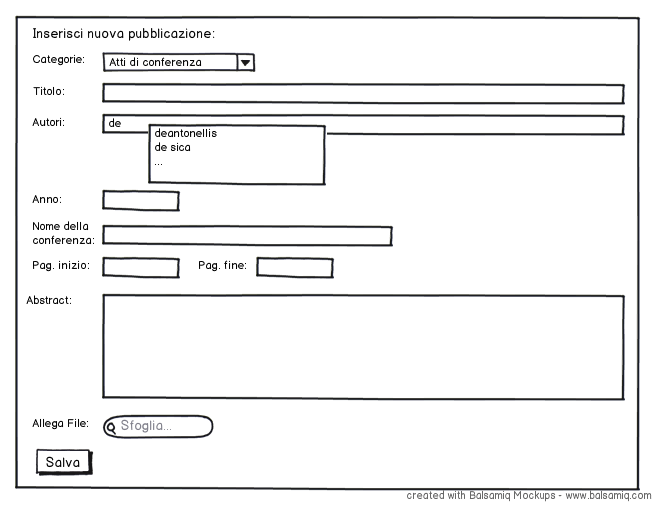
\includegraphics[height=9.5cm]{Mockup/Pubblicazioni/Image/AttiConferenza.png}
\caption{Pubblicazioni in atti di conferenza \label{nome}}
\end{figure}
\\
\textit{Caratteristiche:}
\begin{itemize}
\item Autori: sono da scegliere da una lista che si genera con nuovi inserimenti
\item Nome della conferenza: quando viene visualizzata deve essere preceduta da 'Proc. of'
\end{itemize}
I campi sono tutti obbligatori tranne 'Abstract' e l'allegare un file.
\clearpage

\textbf{4 - Monografia}
\begin{figure}[ht]
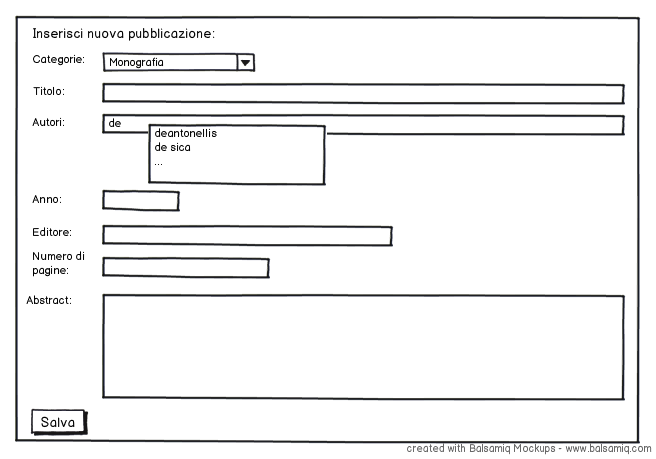
\includegraphics[height=8.5cm]{Mockup/Pubblicazioni/Image/Monografia.png}
\caption{Monografia \label{nome}}
\end{figure}
\\
\textit{Caratteristiche:}
\begin{itemize}
\item Autori: sono da scegliere da una lista che si genera con nuovi inserimenti
\item Editore conterr� sia il nome dell'editore che la citt�
\end{itemize}
I campi sono tutti obbligatori tranne 'Abstract'.
\clearpage

\textbf{5 - Curatela}
\begin{figure}[ht]
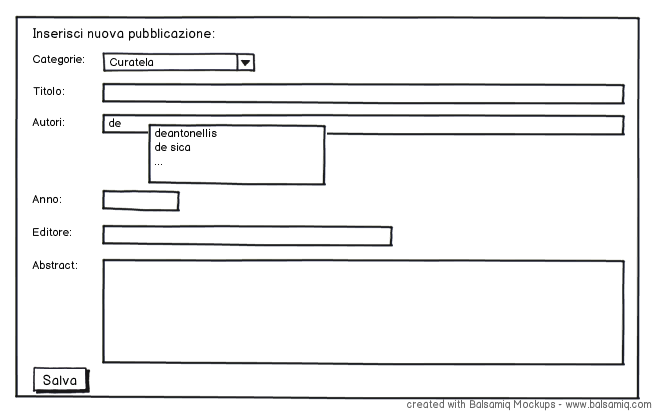
\includegraphics[height=7.5cm]{Mockup/Pubblicazioni/Image/Curatela.png}
\caption{Curatela \label{nome}}
\end{figure}
\\
\textit{Caratteristiche:}
\begin{itemize}
\item Autori: sono da scegliere da una lista che si genera con nuovi inserimenti
\item Editore conterr� sia il nome dell'editore che la citt�
\end{itemize}
I campi sono tutti obbligatori tranne 'Abstract'.

\newpage
\subsubsection{Mockup Corsi}

\textbf{1 - Pagina di creazione e modifica di un corso}
\begin{figure}[ht]
\centering
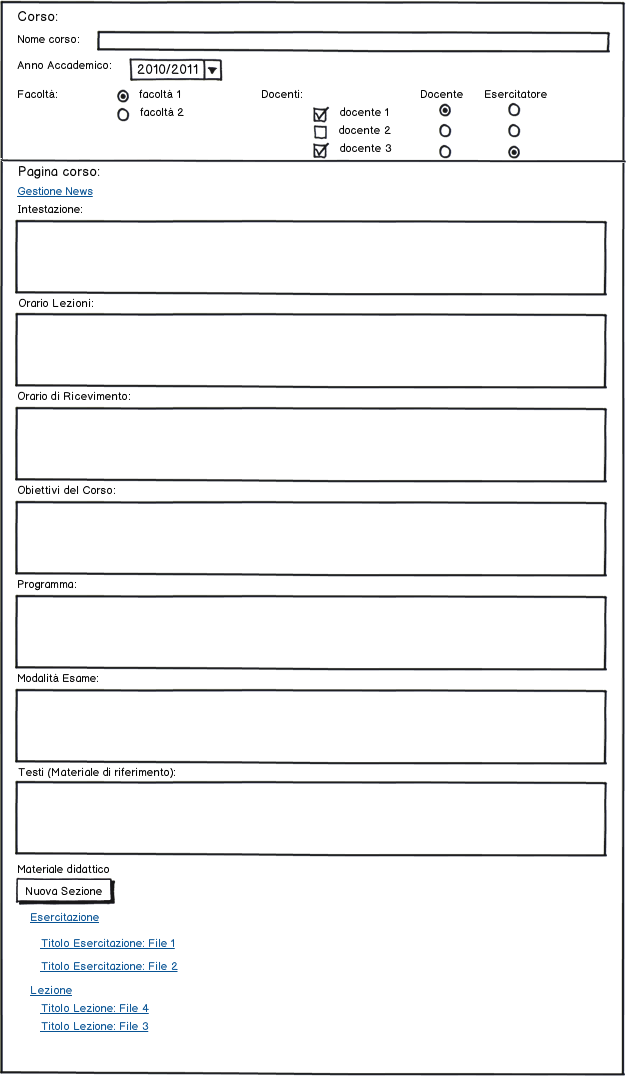
\includegraphics[height=15cm]{Mockup/Corsi/Image/PaginaCorso.png}
\caption{Pagina del corso \label{nome}}
\end{figure}
\\
Pagina per l'inserimento di un nuovo corso e per la modifica di un corso preesistente.\\
\textit{Caratteristiche:}
\begin{itemize}
\item Nome del corso, Anno Accademico, Facolt� e Docenti sono campi obbligatori
\item I restanti campi possono essere alcune volte omessi, quindi il loro inserimento non �
obbligatorio
\item News e Materiale didattico: possono essere inserite solo modificando un corso inserito 
precedentemente
\end{itemize}


\textbf{2 - Gestione News}
\begin{figure}[h]
\centering
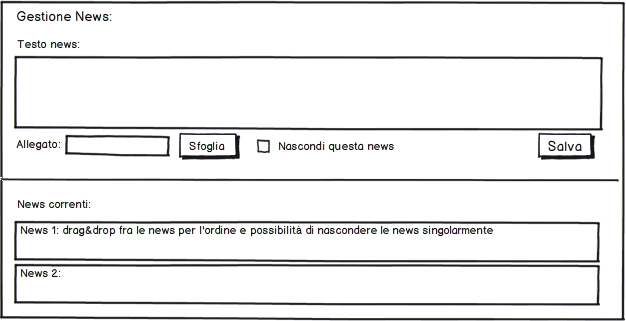
\includegraphics[height=7.5cm]{Mockup/Corsi/Image/GestioneNews.png}
\caption{Gestione News \label{nome}}
\end{figure}
\\
\textit{Caratteristiche:}
\begin{itemize}
\item Le news salvate vengono mostrate nel riquadro in basso 'News correnti', dove l'ordine di tale 
news pu� essere modificato tramite drag\&drop
\item Ogni news pu� essere 'nascosta', in questo modo non apparir� pi� nella pagina web del corso
\item Ad ogni news pu� essere allegato un file
\end{itemize}
\clearpage

\textbf{3 - Materiale Didattico: Sezioni}
\begin{figure}[h]
\centering
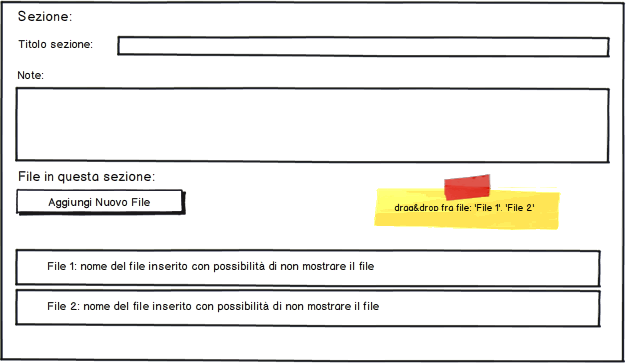
\includegraphics[height=7.5cm]{Mockup/Corsi/Image/Sezione.png}
\caption{Sezione \label{nome}}
\end{figure}
\\
\textit{Caratteristiche:}
\begin{itemize}
\item L'inserimento di una nuova sezione richiede solo il 'Titolo della Sezione',obbligatorio, e il 
campo 'Note' non obbligatorio
\item Una volta inserita una sezione, si ha la possibilit� di aggiungere file a questa sezione, che 
vengono mostrati nel riquadro in basso 'File in questa sezione', dove l'ordine di tale news pu� essere
modificato tramite drag\&drop
\end{itemize}

\textbf{4 - Materiale Didattico: File}
\begin{figure}[h]
\centering
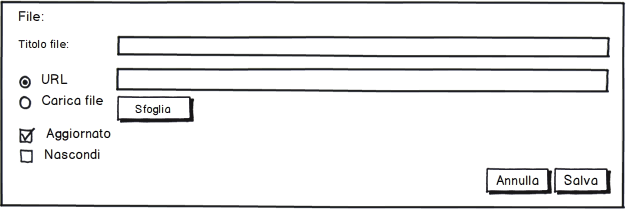
\includegraphics[height=4.5cm]{Mockup/Corsi/Image/File.png}
\caption{File \label{nome}}
\end{figure}
\\
\textit{Caratteristiche:}
\begin{itemize}
\item Ogni file aggiunto avr� un titolo e potr� essere un file caricato oppure un link.
\item Ogni file pu� essere 'nascosto', in questo modo non apparir� pi� nella pagina web del corso, oppure
'aggiornato', in questo modo apparir� nella pagina web con un simbolo particolare in modo da far notare
che � un file caricato di recente, oppure nessuna delle precedenti, in questo modo apparir� semplicemente
il titolo del file nella pagina web del corso.
\end{itemize}
\clearpage

\section{Progettazione della base dati}
\subsection{Progettazione della struttura dati su cui si basa l'applicazione}


\end{document}